\documentclass[nochap,palatino,notitlepage]{apuntes}

\title{Tratamiento de señales visuales - Resumen}
\author{Guillermo Julián Moreno}
\date{15/16 C1}

% Paquetes adicionales
\usepackage{fancysprefs}

% --------------------

\begin{document}
\pagestyle{plain}
\maketitle

\section{Operadores puntuales}

Empezamos definiendo las imágenes como aplicaciones $\appl{ψ}{ℝ^2}{I}$, de tal forma que a cada punto $(x,y)$ le asignan un determinado valor de luminosidad. Para imágenes en escala de grises, $I$ será habitualmente $[0,255]$, aunque también podríamos considerar $I = [0,1]$.

Dada una imagen $ψ(x,y)$ de origen, aplicaremos operadores $\appl{T}{ℝ}{ℝ}$ para obtener imágenes de salida $θ(x,y)$. La convención será que la transformación llevará valores $r_k$ a otros $s_k$.

\subsection{Modelado de histograma}

Este tipo de operadores cambian la amplitud de luminosidad de la imagen y se pueden modelar según su efecto en el histograma de la distribución de posibles valores de luminosidad de los píxeles de la imagen. Se puede normalizar para obtener probabilidades entre 0 y 1. Hay tres operaciones principales con operadores puntuales.

\subsubsection{Ajuste de contraste}

El ajuste de contraste pretende expandir ciertas zonas del rango dinámico y comprimir otros para mejorar el contraste de la imagen. Se define como \[
s = T(r) = \begin{cases}
α r & 0 ≤ r < a \\
β(r-a) + s_a & a ≤ r < b \\
γ(r-b) + s_b & b ≤ r < L - 1
\end{cases}
\]

$α,β,γ$ se calculan según los parámetros $a,b,s_a,s_b$ para que $T$ sea continua. En general, la transformación se puede definir como una transformación lineal en tres intervalos: \begin{align*}
[0, a) &\to [0,s_a) \\
[a, b) &\to [s_a, s_b) \\
[b, L - 1] &\to [s_b, L - 1]
\end{align*}

Un posible puede ocurrir debido a la cuantización: al comprimir ciertos rangos, la aplicación puede dejar de ser inyectiva y entonces será imposible recuperar esa información al restaurar el contraste.

\subsubsection{Igualación de histograma}

La igualación de histograma pretende obtener un histograma lo más uniforme posible. La transformación se define como \[ s = T(r) = \sum_{i=0}^r P(I = i) = P(I <= r) \] donde $P(I = i)$ es la probabilidad de que un determinado píxel de la imagen de entrada tenga valor $i$. En otras palabras, se hace una transformación usando como ``tabla de referencia'' la CDF de luminancia.

Se pueden usar otras funciones como tabla siempre y cuando sean monótonas crecientes. Además, también se puede realizar la ecualización adaptativa realizando el proceso de ecualización en porciones de la imagen. Se puede usar ventana deslizante o bien considerar ventanas con solapamiento.

\subsubsection{Especificación de histograma}

La idea es transformar el histograma de una imagen para que se parezca al de otra imagen. Se hace una correspondencia por percentiles. Sea $F$ la CDF del histograma de la imagen a modificar y $G$ la de la imagen especificada. Entonces, se define la transformación $T$ como \[ s = T(r) = \inf \set{i ∈ [0, L-1] \tq G(i) ≥ F(r) }\]

\subsection{Modificación de niveles}

\subsubsection{Recorte y umbralización}

El recorte sirve para eliminar ruido si se sabe que los niveles de la imagen están en un rango $[a,b]$, llevándolos a un rango final $[s_a, s_b]$. La transformación se define como \[ s = T(r) = \begin{cases} s_a & 0 ≤ r < a \\
α(r - a) + s_a & a ≤ r < b \\
s_b & b ≤ r < L - 1
\end{cases} \] con $α = \frac{s_b - s_a}{b - a}$, esto es, el parámetro que hace que $T$ sea continua.

Cuando $a = b = u$, lo que se realiza es una umbralización, lo que nos permite separar objetos según su luminosidad. El umbral $u$ se puede obtener por un algoritmo iterativo. Dado un umbral $u_i$, se define el siguiente umbral como \[ u_{i + 1} = \frac{\avg{A_i} + \avg{B_i}}{2}\], donde $\avg{A_i}, \avg{B_i}$ son los conjuntos de valores por encima y por debajo respectivamente del umbral $u_i$. El proceso se para cuando la diferencia entre umbrales es menor que uno. El primer umbral $u_0$ se suele tomar como la mitad del rango del histograma, esto es, \[ u_0 = \frac{\max ψ - \min ψ}{2} \]

El umbral se puede seleccionar de forma adaptativa considerando una división de ventanas de la imagen.

Una posibilidad es considerar que la distribución del histograma es una normal bimodal. En ese caso, la PDF es \[ p(r) = P_a p_a(r) + P_b p_b(r) \], siendo $P_a, P_b$ coeficientes de ajuste con $P_a + P_b = 1$. El umbral se definiría como \[ u = \frac{μ_a + μ_b}{2} + \frac{σ_b^2}{μ_b - μ_a} \log \frac{P_a}{P_b} \]

\subsubsection{Negativo, seccionado y extracción de bits}

El negativo es simplemente invertir el histograma, con una transformación $s = T(r) = L - 1 - r$.

El seccionado pretende extraer una determinada banda de niveles sobre el resto. Puede ser extracción o resalte. Respectivamente: \[ s = T_E(r) =
\begin{cases}
s_a & r ∉ [a,b] \\
s_b & r ∈ [a,b]
\end{cases} \qquad
s=T_R(r) = \begin{cases}
r & r ∉ [a,b] \\
s_b & r ∈ [a,b]
\end{cases}
\]

La extracción de bits hace lo que uno podría pensar basándose en el nombre. Los valores cuyo bit $n$-ésimo vale $1$ se transforman a $s_b$, y el resto a $s_a$.

\subsubsection{Compresión logarítmica de rango}

La compresión logarítmica de rango viene dada por \[ s = T(r) = (L - 1) \left(\frac{r}{L - 1}\right)^{\frac{1}{γ}} \]

Si $γ > 1$, se trata de una corrección Gamma, y si $γ < 1$, es corrección Gamma inversa (la respuesta de un monitor CRT, por ejemplo).

\subsection{Aspectos operativos}

Al trabajar con valores discretos, tenemos los problemas habituales de redondeos y truncamientos. Pero además tenemos el problema de que hay que hacer $M × N$ cálculos y operaciones, a pesar de que sólo tenemos $L$ posibles valores de enntrada. En la práctica, se puede o bien modificar la VLT (Video Lookup Table, una tabla de $L$ entradas que relaciona un índice en la imagen con su valor real de colores) o montar una Lookup Table (LUT) con todos los posibles valores de entrada y salida y utilizarla para calcular los píxeles de salida de la imagen final sin tener que rehacer los cálculos.

\subsection{Operaciones aritméticas y lógicas}

Se trata de operaciones aritméticas simples sobre dos imágenes. La resta de imágenes permitirá ver errores, eliminar ruido, detectar movimiento o detectar objetos nuevos o desaparecidos. La suma se puede usar para eliminar ruido de media 0 con un promedio de $N$ imágenes, o también para gestionar transparencias

Las operaciones lógicas también se pueden usar, como por ejemplo, con el operador \textit{AND} para obtener regiones de interés de una imagen.

\section{Operadores LSI}

Los operadores lineales e invariantes con el espacio efectúan transformaciones sobre entornos de píxeles dados. Para eso, se usa una ventana deslizante. Este tipo de operaciones tienen un trasfondo de tratamiento de señal, y vamos a verlo formalmente. Dada una transformación $\appl{T}{M_{2a × 2b}}{[0,L]}$\footnote{$M_{i×j}$ es el espacio de matrices de tamaño $i × j$.} que considera entornos rectangulares $A$ de ancho $2a$ y alto $2b$, podemos considerar la respuesta a un impulso unidad $δ$ de tamaño $2a × 2b$, donde $δ[0,0] = 1$ y vale $0$ en el resto de puntos. Esa respuesta viene dada por $h = T(δ)$. La principal ventaja de esto es que al ser $T$ una transformación lineal, podemos definirla únicamente con esa respuesta, ya que cualquier entorno de la imagen origen será una combinación lineales de deltas desplazadas. Así, la transformación completa $\appl{τ}{M_{M×N}}{M_{M×N}}$ de toda la imagen será \[ θ = τ(ψ) = ψ \ast h \], donde $\ast$ es la convolución, que se define para cada píxel de la siguiente forma: \[ θ[n,m] = \sum_{k=-a}^a \sum_{l = -b}^b ψ[n + k, m + l] \cdot h[-k, -l] \]

Por comodidad, consideraremos $w[n,m] = h[-n, -m]$, invirtiendo la respuesta al impulso $h$ y evitándonos que hacer la inversión en cada cálculo.

Al usar la convolución, podemos irnos al dominio frecuencial. Como notación, las letras minúsculas se referirán al dominio espacial y en mayúsculas al dominio frecuencial, pasando de una a otra con la transformada discreta de Fourier. En el dominio frecuencial, la convolución es un producto y por lo tanto \[ Θ = Ψ \cdot H \], bastante más fácil de computar.

El problema de este tipo de filtros es que nos comemos los bordes al no tener suficientes píxeles para valorar. Para ello, se puede realizar \textit{padding} aumentando la imagen original. Para rellenar esos píxeles adicionales, se pueden usar valores fijos, hacer una simetría, extender el bore con los mismos valores o hacer una réplica circular con el otro lado de la imagen.

La convolución también tiene la propiedad de separabilidad: si nuestro kernel $w$ se puede expresar como $w = x \otimes y$, siendo $\otimes$ el producto de Kronecker y $x,y$ vectores fila y columna respectivamente, entonces aplicar $w$ es lo mismo que aplicar $x$ y después $y$.

Normalmente, para no modificar el valor medio de la luminosidad de la imagen, ponderaremos $w$ para que la suma de sus elementos sea $1$.

\subsection{Tipos de filtros}

Un filtro simple es la correlación: si ponemos como máscara un objeto, la imagen final destacará las zonas donde ese mismo objeto aparezca. El resto son más complejos y merecen secciones aparte.

\subsubsection{Suavizado}

El suavizado es un filtro paso bajo en frecuencia. Sirve para suavizar o emborronar, y se distingue por tener todos los elementos positivos (realiza una media de los píxeles colindantes).

El promedio puede ser ponderado o no ponderado. Un caso especial del ponderado es el binomial, donde consideramos vectores $B_n$ con los coeficientes binomiales, esto es, con $B_n[i] = {n \choose i}$, y con el filtro $w_n = \frac{1}{2^n} B_n \otimes \trans{B_n}$.

El suavizado también se puede hacer con un filtro de mediana, que suele ser más efectivo filtrando ruido tipo sal y pimienta.

\subsubsection{Realce de contornos}

El realce de contornos se relaciona con la primera y segunda derivada direccionales, versión discreta:
\[ \dpa{f[n]}{n} = f[n+ 1] - f[n]\qquad \pd[2]{f[n]}{n} = f[n+1] + f[n-1] - 2f[n]\]

El estudio de la laplaciana (la suma de las derivadas segundas en las dos direcciones) \[ \nabla^2 Ψ = \pd[2]{ψ}{x} + \pd[2]{ψ}{y} \] nos da dos posibles máscaras: la laplaciana $L'$ y la isótropa $I'$, que realzan los bordes:
\[
L' = \begin{pmatrix} 0 & 1 & 0 \\ 1 & -4 & 1 \\ 0 & 1 & 0 \end{pmatrix}
\qquad
I' = \begin{pmatrix} 1 & 1 & 1 \\ 1 & -8 & 1 \\ 1 & 1 & 1 \end{pmatrix}
\]

Normalmente, lo que se quiere hacer es obtener los bordes sin el resto de la imagen, así que las máscaras finales que hacen eso se pueden obtener restando esas máscaras a un único punto obteniendo lo siguiente:
\[
L = \begin{pmatrix} 0 & -1 & 0 \\ -1 & 5 & -1 \\ 0 & -1 & 0 \end{pmatrix}
\qquad
I = \begin{pmatrix} -1 & -1 & -1 \\ -1 & 9 & -1 \\ -1 & -1 & -1 \end{pmatrix}
\]

La Laplaciana nos da la segunda derivada. Para la primera (el gradiente) tenemos varios operadores posibles: Roberts, Prewitt, Sobel y diagonales:
\begin{gather*}
R_1 = \begin{pmatrix} - 1 & 0 \\ 0 & 1 \end{pmatrix} \qquad R_2 = \begin{pmatrix}0 & -1 \\ 1 & 0 \end{pmatrix} \\
P_v = \frac{1}{6} \begin{pmatrix} -1 & -1 & -1 \\ 0 & 0 & 0 \\ 1 & 1 & 1 \end{pmatrix};\,P_h = \trans{P_v}
\qquad
S_v = \frac{1}{8} \begin{pmatrix} -1 & -2 & -1 \\ 0 & 0 & 0 \\ 1 & 2 & 1 \end{pmatrix};\,S_h = \trans{P_v} \\
D^1_1 = \frac{1}{6} \begin{pmatrix} 0 & 1 & 1 \\ -1 & 0 & 1 \\ -1 & -1 & 0 \end{pmatrix};\,D^1_2 = \trans{D^1_1} \qquad
D^2_1 = \frac{1}{8} \begin{pmatrix} 0 & 1 & 2 \\ -1 & 0 & 1 \\ -2 & -1 & 0 \end{pmatrix};\,D^2_2 = \trans{D^2_1}
\end{gather*}

El realce también se puede hacer con filtros diseñados en frecuencia, más concretamente filtros paso alto.

\paragraph{Detección de bordes} La detección de bordes se puede hacer con el realce de contornos. El problema es que los operadores que hemos visto son muy sensibles al ruido, especialmente la laplaciana. Por eso, muchas veces se hace una gaussiana antes (Laplacian of Gaussian)

\subsection{Transformaciones geométricas}

Las transformaciones geométricas mueven los píxeles, normalmente sin cmabiar su valor. Tenemos las transformaciones afines usuales (rotación, escalado, desplazamiento e inclinación) dadas por las respectivas matrices \[
R = \begin{pmatrix} \cos φ & - \sin φ & 0 \\ \sin φ & \cos φ & 0 \end{pmatrix}\quad
E = \begin{pmatrix} ρ_x & 0 & 0 \\ 0 & ρ_y & 0 \end{pmatrix} \quad
D = \begin{pmatrix} 1 & 0 & d_x \\ 0 &  1 & d_y \end{pmatrix} \quad
I = \begin{pmatrix} 1 & -i_x & 0 \\ i_y &  1 & 0 \end{pmatrix} \quad
\]

Para hacer las transformaciones afines, normalmente añadimos un ``1'' al final del vector columna $(x y)$ para poder tener en cuenta los desplazamientos.

Las transformaciones nos permiten corregir distorsiones de la imagen, como la corrección radial o las perspectivas usando proyección geométrica.

\section{Operadores morfológicos}


Los operadores morfológicos implican un tipo de selección distinto al que hemos visto en los LSI. Consideramos dos operadores, supremo ($\vee$) e ínfimo ($\wedge$) y el punto $δ_L(n)$ que vale $0$ cuando $n = 0$ y $- ∞$ en otro caso. Así, una señal cualquiera $x$ se puede representar como \[ x[n] = \bigvee_{k=-∞}^∞ x[k] + δ_L[n-k]\]

\subsection{Dilatación y erosión}

Con el supremo y el ínfimo podemos definir dos operaciones similares a la convolución: la dilatación ($\oplus$) y la erosión ($\ominus$): dado un elemento estructurante $b$, definimos ambos operadores de la siguiente forma para cada punto $y[n]$: \begin{align*}
y[n] = x[n] \oplus b &= \bigvee_{k=-∞}^∞ (x[k] + b[n-k]) \\
y[n] = x[n] \ominus b &= \bigwedge_{k=-∞}^∞ (x[k] + b[n-k])
\end{align*}

\begin{figure}[hbtp]
\centering
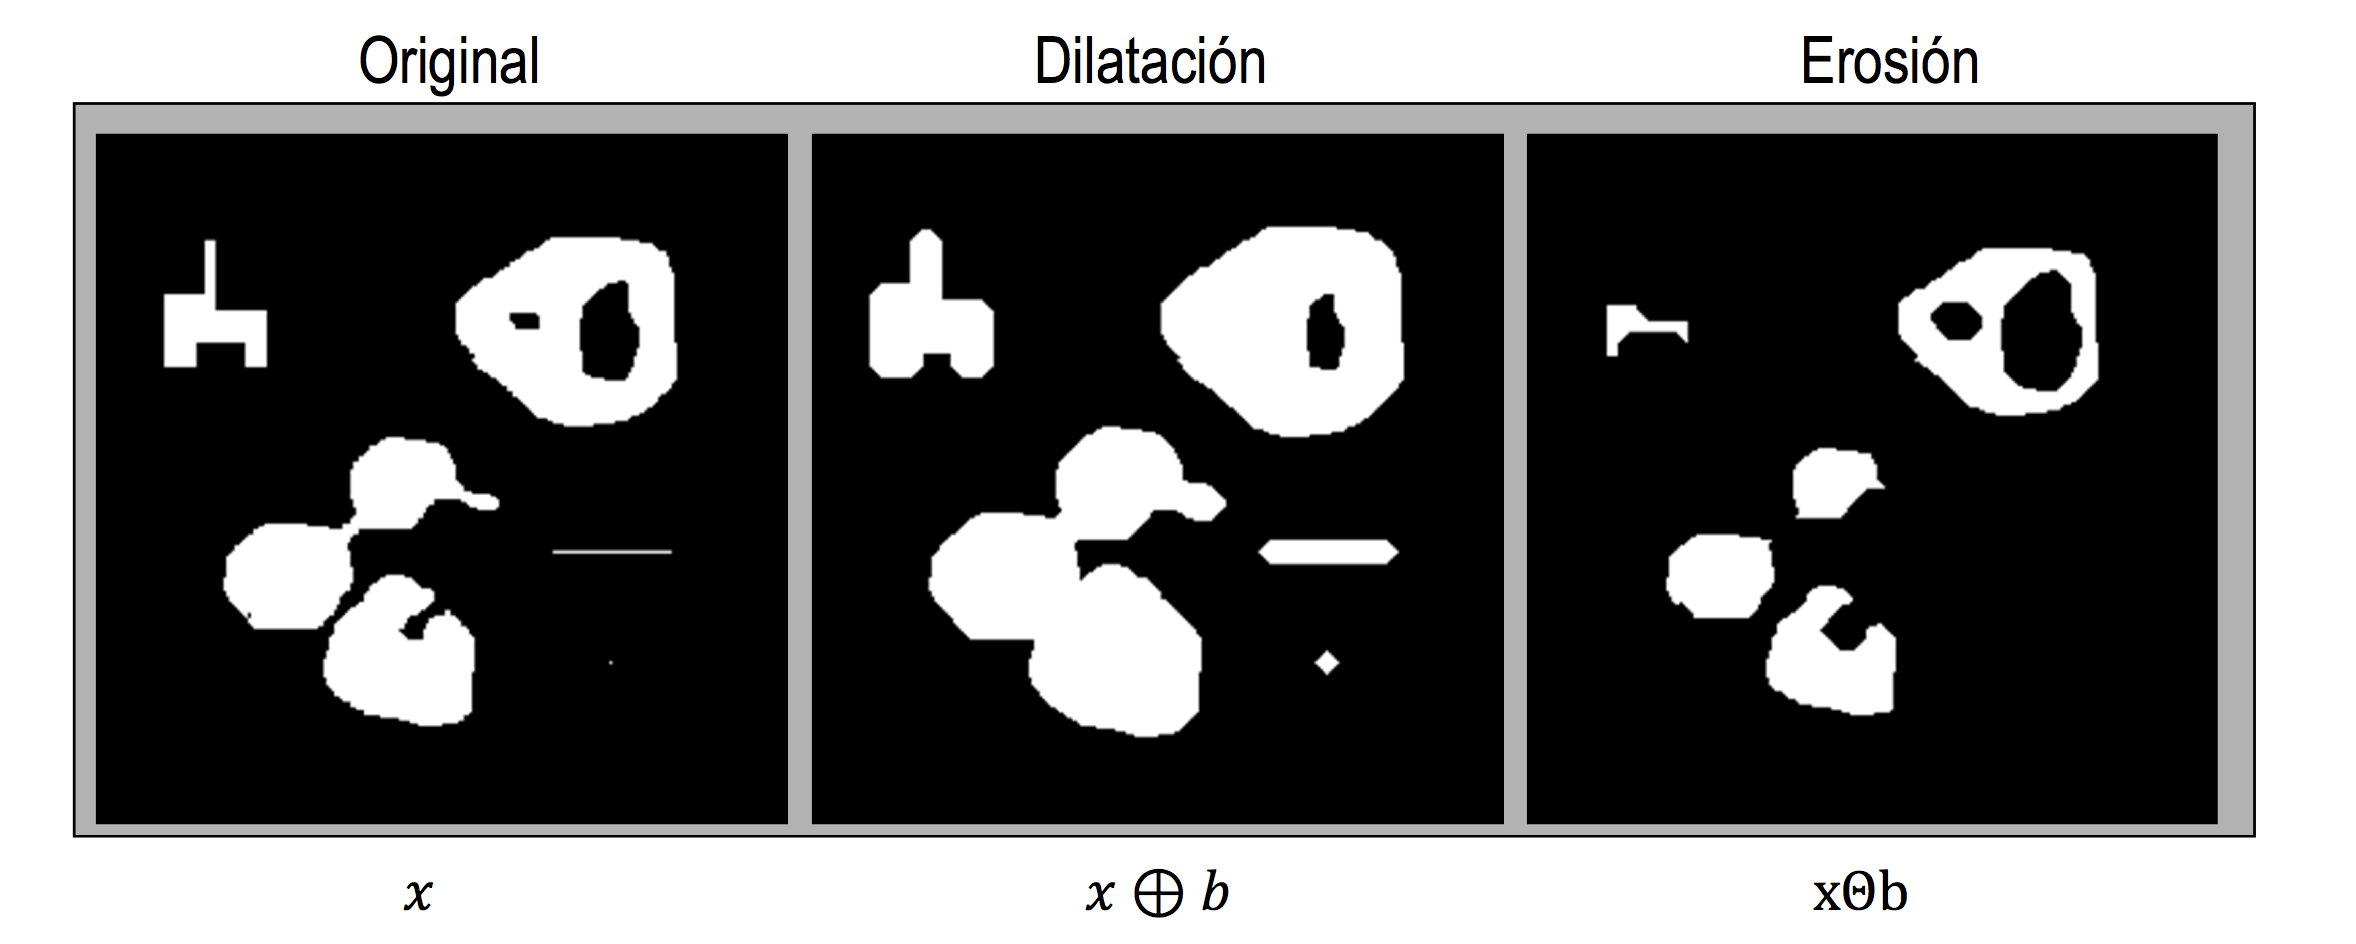
\includegraphics[width=1\textwidth]{img/DilatacionErosion.png}
\caption{Efecto de los operadores dilatación y erosión}
\label{fig:DilatacionErosion}
\end{figure}

En la práctica, la dilatación asigna a un píxel el máximo de todos los píxeles de su entorno que coinciden con los ceros del elemento estructurante invertido. Análogamente, la erosión hace lo mismo pero poniendo el mínimo. El efecto de ambos operadores se puede ver en la \fref{fig:DilatacionErosion}.

La dilatación y la erosión son distributivas con respecto al ínfimo y al supremo:
\begin{align*}
(x \vee y) \oplus b &= (x\oplus b) \vee (y \oplus b) \\
(x \wedge y) \ominus b &= (x\ominus b) \wedge (y \ominus b)
\end{align*}

La composición funciona con la dilatación, pero no del todo bien con la erosión:
\begin{align*}
x \oplus a \oplus b &= x \oplus (a \oplus b) \\
x \ominus a \ominus b &= x \ominus (a \oplus b)
\end{align*}

Si el elemento estructurante incluye el origen, la dilatación es extensiva (los píxeles de salida tienen valor mayor o igual que la entrada) y la erosión antiextensiva (los píxeles de salida tienen valor menor o igual que la entrada).

La dilatación puede reparar objetos, cerrando bordes y quitando imperfecciones (mordidas). La erosión también puede quitar imperfecciones (salidas) y además separar objetos. Ambos operadores pueden ayudar a simplificar imágenes.

\subsubsection{Gradientes morfológicos}

Podemos sacar gradientes por dilatación ($x \oplus b - x$), por erosión ($x - x \ominus b$) o morfológicos ($x\oplus b - x \ominus b$). Si usamos imágenes binarias, deberíamos usar la operación \textit{XOR}.

\subsection{Apertura y cierre}

\begin{figure}[hbtp]
\centering
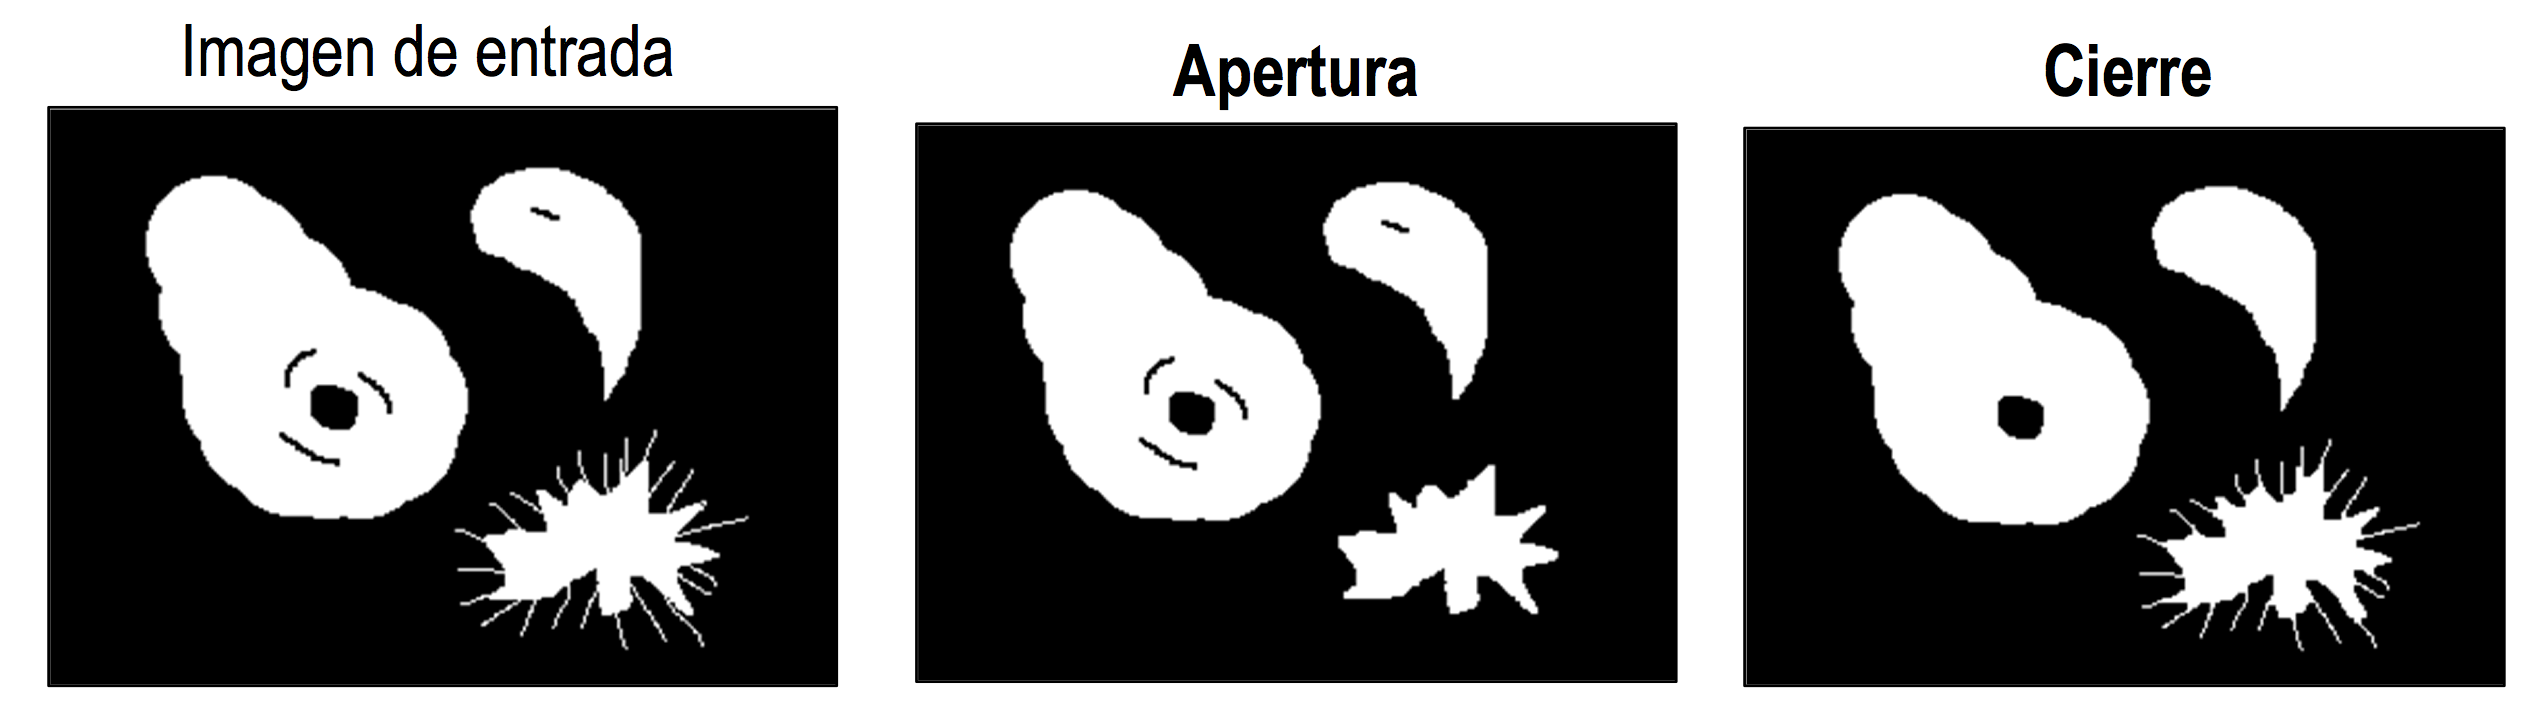
\includegraphics[width=\textwidth]{img/AperturaCierre.png}
\caption{Efecto de los operadores apertura y cierre.}
\label{fig:AperturaCierre}
\end{figure}

Podemos componer los dos operadores básicos para obtener la apertura $γ_b$ y el cierre $φ_b$: \begin{align*}
γ_b &= (x \ominus b) \oplus b \\
φ_b &= (x \oplus b) \ominus b
\end{align*}

El efecto de estos operadores se puede ver en la \fref{fig:AperturaCierre}. La apertura ``abre'' los huecos negros y el cierre ``cierra'' esos mismos agujeros. La apertura es antiextensiva y el cierre extensivo, independientemente de $b$. Además, son idempotentes: sucesivas aplicaciones dan el mismo resultado ($γ(γ(x)) = γ(x)$).

Estos operadores se pueden usar para eliminar objetos de acuerdo a su nivel de gris y de su estructura.

\subsubsection{Detección de objetos}

Se pueden buscar elementos que aparecen como máximos relativos con $x - γ(x)$  (top-hat) y mínimos relativos como $φ(x) - x$ (dual top-hat).

\subsubsection{Granulometría}

\begin{figure}[hbtp]
\centering
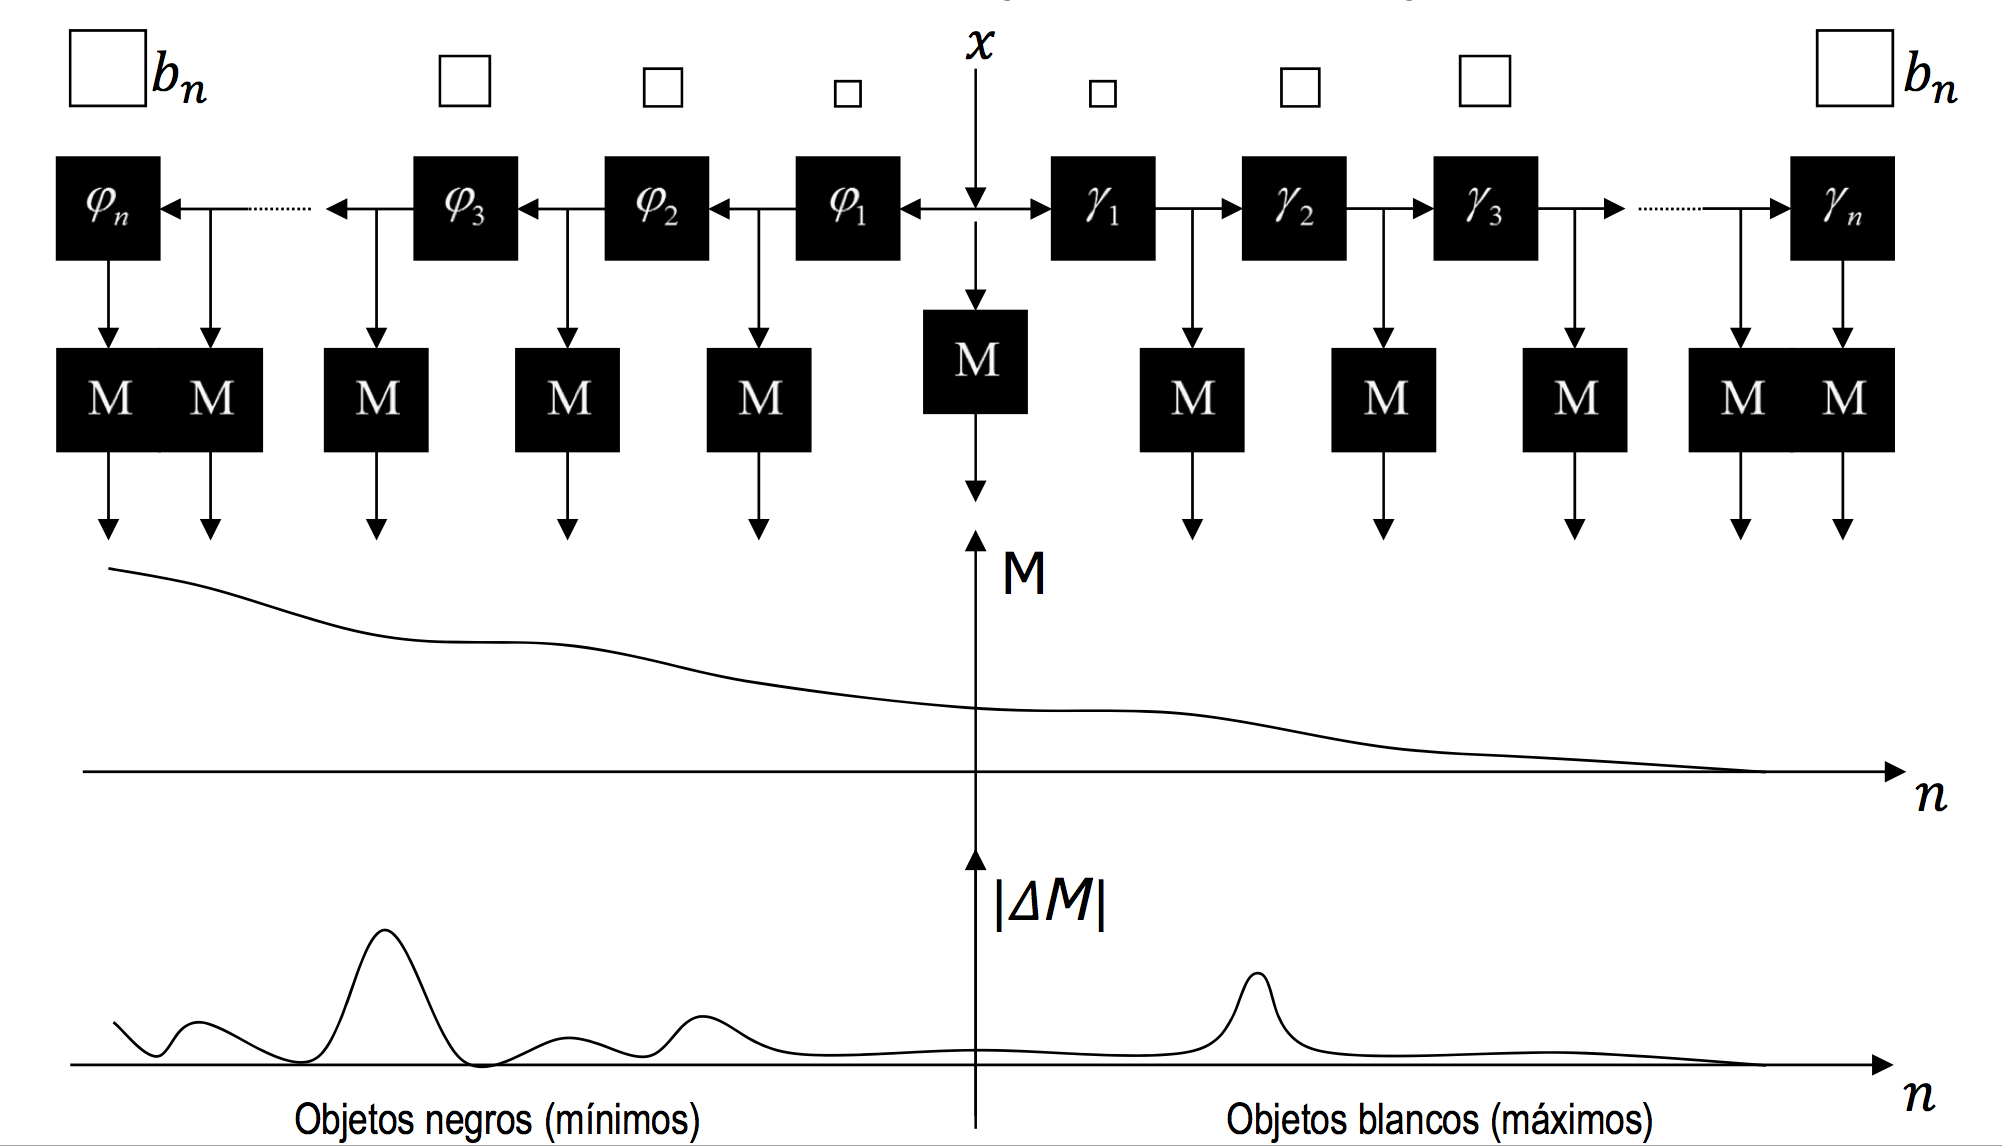
\includegraphics[width=0.9\textwidth]{img/Granulometria.png}
\caption{Granulometría: aplicación sucesiva de aperturas y cierres para detectar cambios en el área.}
\label{fig:Granulometria}
\end{figure}

Aplicando sucesivos bancos de aperturas y cierres (\fref{fig:Granulometria}) con elementos estructurantes crecientes podemos llegar a detectar el tamaño de los objetos.

\subsubsection{Filtrado por reconstrucción}

\begin{figure}[hbtp]
\centering
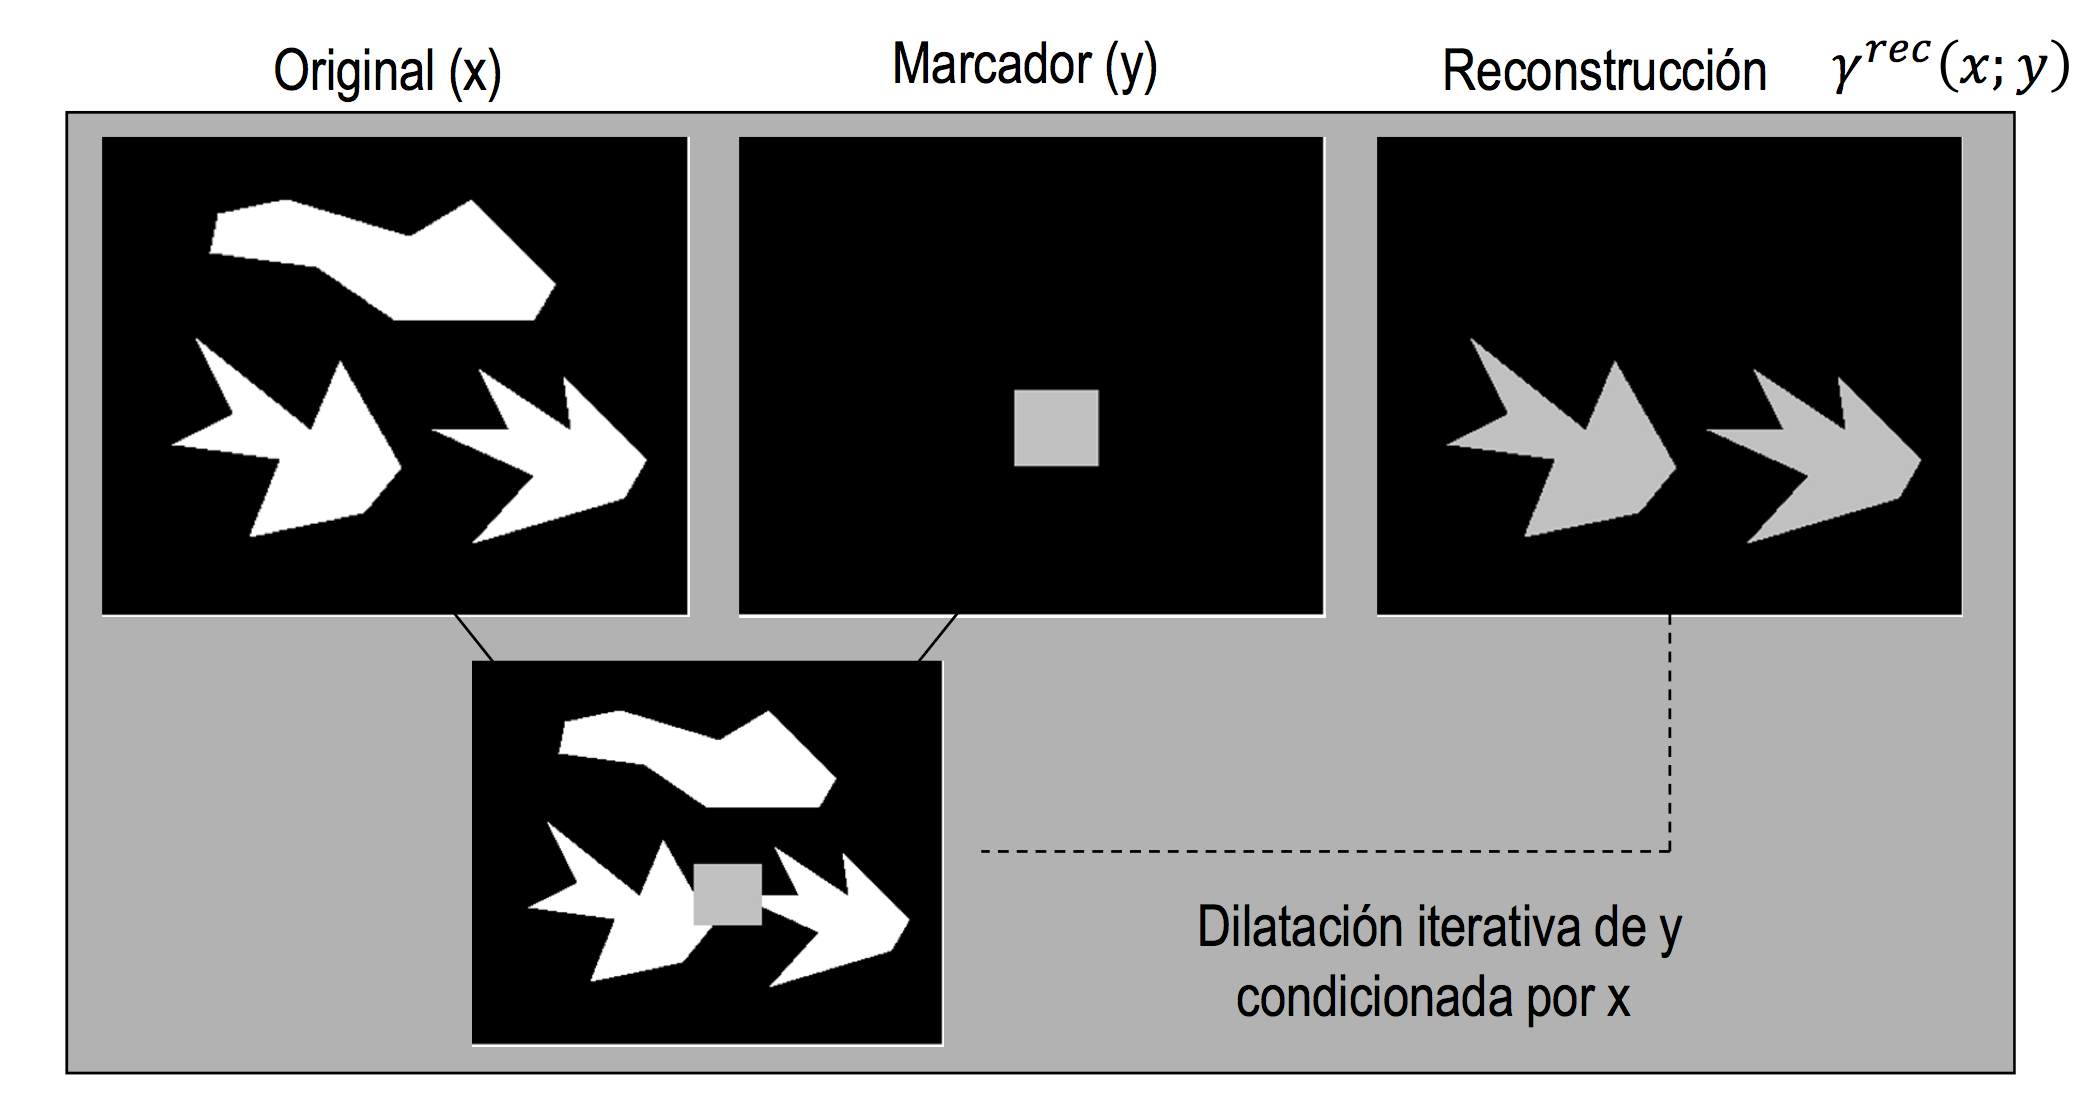
\includegraphics[width=0.9\textwidth]{img/AperturaReconstruccion.png}
\caption{Resultados de la apertura por reconstrucción.}
\label{fig:AperturaReconstruccion}
\end{figure}

Se usan para hacer simplificaciones preservando contornos. Se coge la imagen de entrada $x$, un marcador $y$ y un elemento estructurante que definirá la conectividad de los elementos que mantiene. Se define entonces la apertura y cierre por reconstrucción como un prceso iteratico\begin{align*}
γ^r_i &= (γ^r_{i-1} \otimes b) \wedge x \\
φ^r_i &= (φ^r_{i-1} \ominus b) \vee x
\end{align*} con $γ^r_0 = φ^r_0 = y$. Las operaciones completas se hará con $i \to ∞$, pero por comodidad denotaremos los operadores como $γ^r \equiv γ^r_{∞}$ y $φ^r \equiv φ^r_{∞}$

Tanto la apertura como cierre por reconstrucción tienen las mismas propiedades de extensividad e idempotencia que sus versiones sin reconstrucción.

Normalmente, para el marcador se usarán versiones modificadas de la imagen de entrada, de tal forma que podremos emular la dilatación y erosión sin perder bordes. La apertura mediante reconstrucción de la erosión eliminará ruido más claro que el resto de la imagen, por ejemplo.

También se puede usar este tipo de filtrado para rellenar agujeros, usando un marcador que sea igual a toda la imagen y un cierre por reconstrucción. Un top-hat con la apertura por reconstrucción ($x - γ^r (x;y)$) nos quitará objetos parcialmente visibles si usamos un marcador que sea 1 únicamente en los bordes.

La apertura por reconstrucción de la erosión facilitará el suavizado sin perder los contornos, y el cierre mediante reconstrucción de la dilatación nos permitirá eliminar ruido o elementos pequeños más oscuros sin perder los contornos originales.

\end{document}
